\chapter{Literature Study}\label{lit_study}
In this chapter, an understanding of relevant problems in the current literature is provided. As there is limited work done on routing problems for e-scooters, this chapter describes and compares existing papers discussed similar problems. In the search for relevant articles, Google Scholar has been used as a search tool.

\Cref{PlanningLevels} describes the different planning levels and their decisions in Free-Floating Sharing Systems (FFSS). Within these levels, research done in the field of rebalancing and battery swaps in FFSS is discussed. Due to the connection of the problem to the TOP, an explaination of this problem and existing solution methods is done in \Cref{TOP}. Finally, a summary and comparison of these problems is presented in \Cref{Comparison}, before \cref{Conclusion} gives a motivation for the report.


\section{Planning Levels in Free-Floating Sharing Systems}\label{PlanningLevels}

E-scooter Sharing Systems (ESS) are a type of free-floating systems that are characterized by vehicles that can be picked up and parked where the user wants. \citet{mckenzie_spatiotemporal_2019} points out that research regarding free-floating ESS is concentrated around social impact, parking placement, adoption rates, and safety concerns. Therefore, a study of similar research to ESS is examined. Similar research fall into the categories of Electrical Bike-Sharing Systems (EBSS), Free-Floating Bike Sharing Systems (FFBSS), and the more general Free-Floating Shared Systems (FFSS).  

As for general FFSS, optimization problems regarding ESS can be divided into three levels; the strategic level, tactical level, and operational level. Decisions made at each level help shape the entire system towards optimal decision-making. The strategic level is the foundation of the system and for an ESS it deals with decisions related to the business model or the infrastructure of the business, i. e. pricing, incentive schemes, marketing, e-scooter types, number of e-scooters, and detecting user demand. The output from the strategic level works as unchangeable input to the tactical level, where decisions regarding inventory distribution, optimal allocation, and detection of damaged e-scooters are made. The strategic and tactical decisions generate the input of the operational level. The operational level deals with daily operations including the rebalancing of the e-scooter fleet and battery replacement. 

The interdependence of the different planning levels in the ESS is shown in \Cref{fig:planning}. The decisions from the parent levels work as input for the child levels decisions. 
\\
\begin{figure}[H]
    \centering
    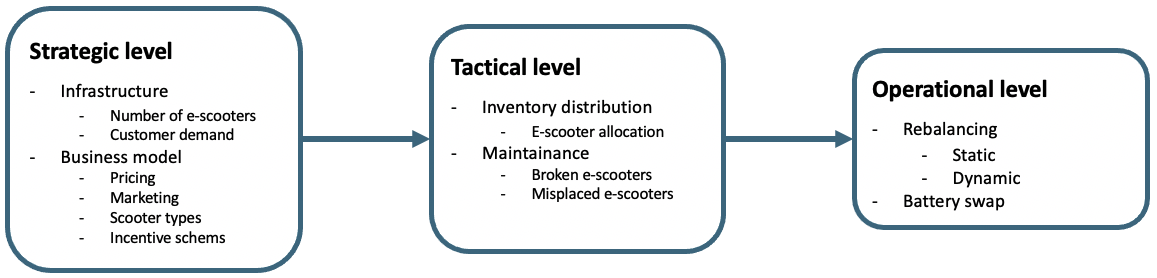
\includegraphics[width=1\columnwidth]{Images/planning_levels.png}
    \caption{Planning levels in free-floating sharing systems}
    \label{fig:planning}
\end{figure}

\subsection{The Strategic Level}\label{strategic}
The strategic decisions of an ESS involve the infrastructure and business model of the operators. The decisions are often made before an operator enters the market, and require capital investments. Once made, these decisions stay unchanged for a longer period of time. However, strategic decisions regarding the e-scooters are often remade every year, as there is a need to replace the e-scooters with new and improved ones every now and then. This is opposed to most other industries, where the strategic decisions are made less frequently. This is a result of the e-scooter market being young and dynamic, requiring operators to constantly pay attention to market needs and customer demand, and adapt accordingly. 

The decisions related to infrastructure in strategic planning mainly involve analysis of customer demand and competition in order to determine the optimal number of e-scooters to allocate around a city. Further, it is important to analyze the geographical peculiarities and the interplay between users and other transportation modes in a city. \citet{templ_fleet_2020} has developed a management tool that describes important information about past, present, and future vehicle counts in FFBSS. They have formulated a Markov Chain Model to integrate information about service level and the geographical distribution of vehicles facilitating the strategic decisions related to demand analysis. 

\citet{he_operations_2019} discuss the effect of the fleet size in a free-floating system. Using a two-stage stochastic optimization model developed by \citet{lu_optimizing_2017} and data from the Boston-Cambridge area, they conclude that a larger fleet size improves the systems profitability and quality of service substantially. This is backed by \citet{ciociola_e-scooter_2020} which stress the importance of a large fleet to increase customer satisfaction.

Another important decision on the strategic level is pricing and incentive schemes. Incentive schemes directed at achieving natural rebalancing can greatly influence the decisions at the tactical and operational levels. \citet{lu_considering_2019} study these schemes in the light of FFBSS. They combine big data and spatial agent-based modeling to achieve results indicating that a discount of at least 30\% would make users of sharing systems change their parking location. This result suggests that a zone-based drop-off of e-scooters also could be feasible for ESS, reducing operational costs. 

A second incentive system, developed by \citet{heitz_designing_2020}, could reduce the impact of the research conducted by He, Miaojia Lu, Ciociola and their respective coauthors. Focusing on EBSS, \citet{heitz_designing_2020} have used operational research to assess different options for incentive systems with respect to the value creation both for operators and users. The result is an incentive system that allows reducing the number of e-bikes by 30\% without diminishing the service level. Users of the service are rewarded for dropping off their bikes in dynamically changing reward zones whose locations are based on the bike distribution and the future demand pattern. Thus, by using this incentive scheme it is reasonable to think that ESS operators also could reduce the amount of e-scooters required to satisfy the demand. 

Decisions regarding the business model of companies operating fleets of e-scooters are definitively important for the success of those companies, but will not be researched further in this report. 

\subsection{The Tactical Level}

The output from the strategic level works as an input to the tactical level. At this level, the aim is to make the best use of the resources allocated from the strategic level, in order to yield the highest possible service level given user demand patterns (\cite{paias_service_2016}). The tactical level contains decisions regarding the allocation of the e-scooter fleet, as well as maintaining the availability of the fleet. The allocation should compensate for variations in demand during the course of a day. In order to do this successfully, thorough demand and use pattern forecasts are necessary. 

\citet{jiao_understanding_2020} has studied the demand and user behavior of the e-scooter market in detail. Using Austin, Texas, as the point of focus, they have analysed travel patterns from over 1.7 million e-scooter trips from 2018 and 2019. Their results show that areas with higher population density naturally has led to more e-scooter trips, but also that areas with higher educated citizens are correlated with increased use of micromobility services. Furthermore, shorter distances to the city center, better street connectivity, and the presence of transit stations are also factors associated with increased usage of e-scooters. Surprisingly, the proportion of young residents within a neighborhood has been proven negatively correlated with e-scooter usage. All these contributions are important to take into account when making decisions at the tactical level.

As most of the work done on ESS has been concentrated around social impact, parking placement, adoption rates, and safety concerns, the allocation of the e-scooters has not been given a substantial focus. However, if a parallel is drawn between bike sharing stations and zones or areas in a city, some of the research done on FFBSS and EBSS is relevant for ESS as well. Finding the ideal state for geographical zones is relevant for different sharing systems. \citet{vogel_service_2016} utilizes data mining techniques to get insight into use patterns of sharing systems, after which an ideal state for different stations was determined. \citet{schuijbroek_inventory_2017} model the stochastic demand at stations using a queuing system and Markov chains to determine ideal states. \citet{paias_service_2016}, on the other hand, assume that the user demand is more deterministic, and exhibits similar patterns each day. The ideal state of a station is then limited by a fixed absolute value for the mismatch between the initial and final state.

\subsection{The Operational Level}
The operational level takes the decisions from the strategic and tactical level as given, and aims to optimize the everyday operations. In ESS, decisions related to everyday operations are divided into three main aspects: rebalancing of e-scooters, battery swaps and generation of routes for service vehicles. 

\subsubsection{Rebalancing}

In their 2017 research paper, \citet{lu_optimizing_2017} stress the importance of rebalancing in sharing systems. As one-way demand increases, the number of rebalancing trips follows. The rebalacing problem becomes significantly more difficult to solve when the free-floating aspect is introduced to the sharing systems. \citet{pal_free-floating_2017} divide the problem into two: user-based strategies and operator-based strategies. The user-based strategies deal with incentive schemes and pricing programs aimed at achieving natural rebalancing, as discussed in \Cref{strategic}. Operator-based strategies focus on the use of service vehicles to manually rebalance the sharing systems, which is the content of this section. The rebalancing problem can either be static or dynamic, depending on whether or not user interference is considered in the problem.  

The static rebalancing problem is well-studied for sharing systems. \citet{pal_free-floating_2017} have developed a Novel Mixed Integer Linear Program for solving the Static Complete Rebalancing Problem for FFBSS, which is highly transferable to the rebalancing problem for ESS. Their model can handle multiple service vehicles and is efficient for solving rebalancing problems for large-scale bike sharing systems. \citet{liu_static_2018} look into the same problem for FFBSS. They also consider multiple heterogeneous service vehicles and use an enhanced version of chemical reaction optimization to solve the problem. Their results provide a model that can tackle the rebalancing problem for larger instances, longer rebalancing durations, and more vehicles than previously proposed models. Further research is done by \citet{du_static_2020}, which focus on the static rebalancing of malfunctioning bikes in a FFBSS. They develop a greedy-genetic heuristic that proves effective for solving large instances of their integer linear programming problem. 

 \citet{caggiani_modeling_2018} propose a dynamic redistribution methodology similar to the the dynamic rebalancing problem. They start from a prediction of the demand over an operating area and end up with a relocation decision support system. Their relocation process is rerun at a constant time gap in order to carry out dynamic bike redistribution. This achieves a high level of user satisfaction while minimizing the cost of operating the service vehicles. 

\subsubsection{Battery swap}

The battery swap procedure is largely dependent on the battery level of the e-scooters and the number of service vehicles available. Developing viable schemes for this procedure is a field of research that has not been explored deeply. There is, however, some research done on alternative battery charging schemes and evaluation of battery life. 

\citet{pender_stochastic_2020} have developed a stochastic model to capture the battery life dynamics of e-scooters of a large network. They have developed an algorithm for determining the number of service vehicles that are needed to guarantee the desired levels of performance of the system. However, this research is based on the sharing system used in the USA where individuals perform the battery swaps, rather than service personnel hired by the operators.

\citet{schnieder_evaluation_2019} discusses the technical requirements of electric sharing systems. They explore the additional workload of these systems compared to conventional bike sharing systems by simulating different charging schemes based on real-life data. Among different battery swapping scenarios explored by Schnieder and West are scenarios looking into battery swapping during relocation trips during the night when the user interference is negligible.  

\citet{fosen_rebalancing_2020} explores the utility of battery swapping by means of service vehicles in EBSS. They discuss the combination of rebalancing and battery swapping and provide a model designed to provide optimal routes for service vehicles performing operations in a EBSS. Many of their findings are highly applicable to problems in ESS as well.  

\textbf{Efficient route planning for service vehicles}

Based on the aspects discussed above, it is necessary to develop efficient routes for the service vehicles to take while performing rebalancing moves and battery swaps in FFSS. These route planning problems fall into the combinatorial optimization and integer programming problem category (\cite{fosen_rebalancing_2020}). Given the nature of the combination between rebalancing and battery swap execution, the problem discussed in this report can further be modeled as a variant of a Team Orienteering Problem, which is discussed further in the following section. 


\section{Team Orienteering Problem}\label{TOP}
This section describes the Team Orienteering Problem (TOP) and presents some methods for solving it.

\subsection{Description of the Problem}

The team orienteering problem is a variant of the more general Orienteering Problem (OP) (\citet{gunawan_orienteering_2016}). The OP consists of a vehicle with a limited time frame and a set of nodes, each with a reward assosiated with it. The vehicle is able to visit the nodes by traveling between them. For every node visited, a reward is given, and the overall goal is to maximize the total reward given by only visiting each node once. Additionally, a time constraint prohibits the vehicle from visiting all nodes, and a selection is necessary. The OP can therefore be seen as a combination of the knapsack problem and the traveling salesman problem \citep{vansteenwegen_orienteering_2011}.

The problem is better understood by studying the origin of the name of the problem, i.e.  the sports game of orienteering (\cite{chao_team_1996}). In a score orienteering event, the contender is given a map of posts to visit with a corresponding reward associated with visiting each post (\cite{tsiligirides_heuristic_1984}). The goal of the sport is to achieve the highest reward possible given a limited time frame. The winner of the tournament will not necessarily visit all posts, but prioritize the posts given the time needed. \Cref{fig:TOP} shows a possible solution to the orienteering problem. In this example, there is a time constraint of 30 minutes for illustration purposes. The bold lines between the nodes illustrate the chosen path. Posts 1 and 4 are not visited as the time needed to reach them is too long given the time constraint. If, for example, node 4 had a big reward associated with it, the route might prioritize this one, and we would get a different route.

\begin{figure}[h]
    \centering
    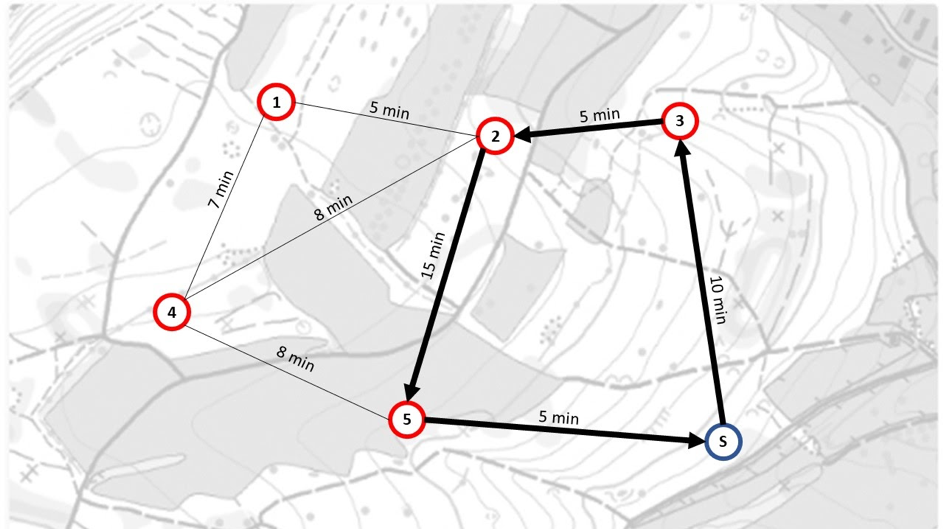
\includegraphics[width=12cm]{Images/TOP.png}
    \caption{Example solution to the Orienteering Problem}
    \label{fig:TOP}
\end{figure}
\break
The TOP problem is the basis of the problem of this report and simply an extension of the OP. In the TOP, several paths is determined with each path having their time frame. However, each node can only be visited once. This is similar to having a team participate in the sports game of orienteering, hence the name. The TOP is an interesting problem for this report due to the ability of not choosing to visit every single node. In the real world setting, there is not enough time to swap batteries and rebalance every e-scooter. The model should prioritize the most important ones which yield the highest reward. 

\subsection{Solution Methods}\label{lit_solution_methods}

The OP is generally a hard problem to solve. It is proven to be an NP-hard problem (\cite{golden_orienteering_1987}), implying that no polynomial-time algorithm has been designed to solve it. Consequently, heuristic methods are used to solve the practical application-sized problems. However, the problem is still challenging to solve using heuristics. \citet{gendreau_tabu_1998} argue that it is hard for a heuristic to pick nodes that are part of the optimal solution. This is due to the independence of the reward for visiting a node and the time it takes to get there. Hence, it is difficult for a heuristic algorithm to efficiently explore the solution space and navigate in the right direction. Additionally, some problem instances are harder to solve than others. \citet{vansteenwegen_iterated_2009} found that instances where the optimal number of visited vertices were a little over half of the total number of vertices was the most difficult to solve. This is due to the high number of vertices that need to be evaluated in these cases and the general high complexity of solving a larger problem. \citet{chao_team_1996} has created a set of benchmark instances which is used to compare different solution methods. The number of nodes in these instances vary from 21 to 102 with the number of vehicles varying between 2, 3 and 4.

Exact algorithms for solving the TOP have been published by \citet{butt_optimal_1999}, \citet{boussier_exact_2007}, \citet{poggi_team_2010}, \citet{dang_effective_2013}, and \citet{keshtkaran_enhanced_2016}. \citet{butt_optimal_1999} have used a column generation algorithm solving instances up to 100 vertices. In combination with column generation, \citet{boussier_exact_2007} and \citet{keshtkaran_enhanced_2016} have used branch-and-bound to create a branch-and-price scheme. In addition to the branch-and-price scheme, \citet{boussier_exact_2007} have used several acceleration schemes to find the optimal solution faster. \citet{keshtkaran_enhanced_2016} have based their model on the work by \citet{boussier_exact_2007}, adding relaxations and valid inequalities to the pricing problem. Other exact algorithms have been adding cutting planes to the algorithm (\cite{dang_effective_2013}; \citet{poggi_team_2010}). \citet{poggi_team_2010} have used a branch-and-cut-and-price algorithm, solving the pricing sub-problem by Dynamic Programming, while \citet{dang_effective_2013} have introduced a branch-and-cut scheme. They introduce a set of dominance properties, valid inequalities, and symmetry-breaking constraints making the model competitive with other methods of the literature.

\citet{chao_team_1996} were the first to publish a heuristic method for the TOP. They presented a five-step heuristic looking only at the nodes that can be reached. They initialize many different paths with one node far away from the depot, choose the best ones, and apply four improvement steps to make the solution better. Later, \citet{archetti_metaheuristics_2007} and \citet{vansteenwegen_iterated_2009} created variable neighborhood search algorithms. \citet{archetti_metaheuristics_2007} were able to achieve very low optimality gaps. They used a combination of a tabu search and a variable neighborhood search. This was done by jumping to intermediate solutions, improving it by tabu search, and then comparing it to the old solution. If the new solution is better, they continued with that one. \citet{vansteenwegen_iterated_2009} were able to achieve a computational time of only a few seconds for the big instances of 100 nodes. They implemented a Skewed Variable Neighborhood Search (SVNS) framework having different mechanisms for exploring new solutions and optimizing current solutions. \Cref{fig:ComparisonSolutionTOP} summarizes solution methods developed to solve the TOP.
\\
\begin{table}[H]
    \centering
    \caption{Summary of different solution methods for TOP}
    \begin{tabular}{ c c c } 
         \hline
             Reference & Algorithm & Exact/Heuristic \\ 
        \hline
             \citet{butt_optimal_1999} & Column Generation & Exact \\ 
             \citet{boussier_exact_2007} & Branch-and-Price & Exact \\
             \citet{poggi_team_2010} & Branch-and-Cut-and-Price & Exact \\ 
             \citet{dang_effective_2013} & Branch-and-Cut & Exact \\ 
             \citet{keshtkaran_enhanced_2016} & Branch-and-Price & Exact \\ 
             \citet{chao_team_1996} & Five Step heuristic & Heuristic \\ 
             \citet{archetti_metaheuristics_2007} & Variable Neighborhood and Tabu Search & Heuristic \\ 
             Vansteenwegen et. al. (2009) & Variable Neighborhood Search & Heuristic \\ 
        \hline
    \end{tabular}
    \label{fig:ComparisonSolutionTOP}
\end{table}

\section{Comparison of Relevant Studies}\label{Comparison}

The primary purpose of this chapter is to place the report within the research conducted. In this section, a comparison of research that mainly focuses on the rebalancing and battery swaps of FFBSS is conducted. \Cref{comp_study_overview} presents the studies conducted for comparison in this report. The selected studies for the comparison is based on the ones deemed relevant for the scope of this report and their characteristics are summarized in \Cref{comp_study_matrix}.
\\\
\begin{table}[H]
    \centering
    \caption{Research conducted for the comparison study}
    \begin{tabular}{c| l}
        \# & Article \\
        \hline
        1 & \citet{caggiani_modeling_2018}\\
        2 & \citet{pal_free-floating_2017}\\
        3 & \citet{warrington_two-stage_2019}\\
        4 & \citet{du_static_2020}\\
        5 & \citet{liu_static_2018}\\
        6 & \citet{pender_stochastic_2020}\\
        7 & \citet{ciociola_e-scooter_2020}\\
        8 & \citet{masoud_heuristic_2019}\\
        9 & \citet{fosen_rebalancing_2020}\\
    \end{tabular}
    \label{comp_study_overview}
\end{table}

\subsection{Objective Function}\label{comparison_oj_func}

Optimization research concerning free floating systems like FFBSS and ESS focuses on two main objectives, minimizing costs and maximizing customer utility. \citet{caggiani_modeling_2018}, \citet{ciociola_e-scooter_2020}, and \citet{fosen_rebalancing_2020} either minimize the unmet demand or maximize customer utility. Objective functions that minimize cost either reduce operation time or travel distance for the operators while forcing user demand or a rebalancing schema to be fulfilled. This applies for \citet{pal_free-floating_2017}, \citet{warrington_two-stage_2019}, and \citet{masoud_heuristic_2019}, whereas \citet{liu_static_2018} model a combination of the two aspects. 

\subsection{Demand}\label{comparison_demand}

The expected demand for the different models is either based on analysis of historical data, a statistical prediction based on a distribution that mirrors the user demand, or data models such as neural networks trained on historical data. Analysis of historical data is the most used demand prediction tool  \citep{pal_free-floating_2017, du_static_2020, liu_static_2018, pender_stochastic_2020, masoud_heuristic_2019, fosen_rebalancing_2020}. \citet{warrington_two-stage_2019} use Monte Carlo simulations with different scenarios while  \citet{caggiani_modeling_2018} trains a neural network on historical data and then use the neural network to predict demand.

\subsection{Solution Method}\label{comparison_modl_meth}

As the research on ESS is quite limited, the area of FFBS and general shared mobility systems is looked at to understand the field of relocation in free floating systems. Rebalancing in FFBS is studied both for the static and dynamic case. For the static case, the use of heuristics is proven to be effective to solve real-life instances \citep{pal_free-floating_2017, du_static_2020, liu_static_2018}. For the dynamic case, a two-stage stochastic programming has been applied by \citet{pal_free-floating_2017} and \citet{fosen_rebalancing_2020}. 

The Team Orienteering Problem fulfills some of the characteristics of the problem of this report. The operators are not able to rebalance and swap all e-scooters during a night shift. Hence, the system has to prioritize which e-scooters to manage or not. Several solution approaches are presented in \cref{TOP}. The most promising are looking at cutting plane schemes, and special neighborhood search heuristic algorithms.

\subsection{Main Decision}\label{comparison_main_decision}

This report studies articles on rebalancing and general routing for free floating systems. To the best of the authors knowledge, there has been limited amount of research on battery swapping for ESS. Simulations of required “swappers” per e-scooter performed by \citet{pender_stochastic_2020} and simulations on how different system variables affect ESS done by \citet{ciociola_e-scooter_2020} are some of the latest research in the field of ESS looking at battery swapping. The research by \citet{masoud_heuristic_2019} on assigning "swappers" to e-scooters is somewhat different from the problem of this report, as these “swappers” are private persons and not a company performing the battery swapping. 


\import{./Tables/}{Literature review comparison table}

% TO DO!!!!
\pagenumbering{arabic}
Helt TOP!
\newpage
\setcounter{page}{25}

\section{Conclusion and Motivation of the Report} \label{Conclusion}

Micromobility sharing systems have received increasing attention in the last decade. The main focus of research on the topic is, however, on BSS. Some research has been done on FFBSS and EBSS, but the problems related to e-scooters are rarely addressed. Thus, this chapter looks at the literature on different sorts of free-floating systems and aims at understanding the degree of relevance this research has for ESS. 

The main focus of the literature study is on the operational level, including rebalancing, battery swapping, and service vehicle routing. Rebalancing schemas have been discussed to some degree in previous literature, but unfortunately the models designed are aimed at bicycle systems, and do not take the dynamics of ESS into account. When it comes to battery swaps, the literature is limited, both for FFBSS and ESS. This is a result of battery swaps being a relatively new concept. Thus, this report will handle the action of battery swaps for e-scooters in a way not previously explored.

The combination of rebalancing and battery swaps has, to the authors knowledge, been left undiscovered in optimization research for ESS. While research has been conducted on rebalancing moves and vehicle routing for sharing systems, the combination of the actions is a new approach to ESS. Hence, this report explores areas of operations research on sharing systems, not previously given much attention. This is backed by feedback from the two major operators of ESS in the Norwegian market, which has expressed that they see great potential in the problem discussed in this report. 

Additionally, the possibility of not visiting all vehicles that are in need of assistance has not been given much attention. Most models designed for optimizing vehicle routing in sharing systems have been designed to visit all shared vehicles that need manual attendance. Consequently, this report determines a set of routes for service vehicles performing both rebalancing and battery swaps, but not necessarily visiting every node in the network. The TOP is closely related to this type of problem, allowing for a selection of shared vehicles to be handled including a vehicle routing problem. Hence, the TOP and its corresponding solution methods are emphasized in this literature review.

Inspired by the work conducted on rebalancing and vehicle routing for FFSS, this report presents a mathematical formulation to address routing for service vehicles operating in an ESS. Optimal routes are created in order to increase the availability of the fleet of e-scooters. This will further increase the customer benefit of the system, as well as reducing the operational costs for the operators of the systems.  
